\documentclass[letterpaper,12pt,dvips]{book}
% Para un buen acomodo en 11 pts.
%\hoffset=-1cm  
%\voffset=-3cm
%\textheight=22cm
%\textwidth=16cm
%\parindent=0cm
%\parskip=0.2cm

% Para un buen acomodo en 10 puntos y lasertjet Hp.
%\hoffset=-1.6cm  
%\voffset=-1.5cm
%\textheight=22cm
%\textwidth=16cm
%\parindent=0
%\parskip=0.2cm

% Para un buen acomodo en 12 puntos y report. ---------------------------
%\hoffset=-1.2cm  
% \voffset=-1cm
 %\textheight=22cm
 %\textwidth=16cm
 \parindent=0cm
 \parskip=0.2cm

% En la version vieja del libro de jaime
% \hoffset=-1.8cm  
% \voffset=-2.5cm
% \textheight=24cm
% \textwidth=17cm
% \parindent=0cm
% \parskip=0.2cm

%------- Page layout for lettersize -------------



\usepackage[utf8]{inputenc}
\usepackage[spanish,activeacute]{babel}

%\usepackage{rotating}   % Para rotar tablas.
\usepackage{array}      % Para hacer tablas raras.
%\usepackage{epsfig}
\usepackage{makeidx}
\usepackage[pdftex]{graphicx}

%\usepackage{amstex}      % Debe estar despues de babel !!!
\usepackage{amsmath}      % Debe estar despues de babel !!!
\usepackage{amssymb}      % Debe estar despues de babel !!!
\usepackage{bm}           % Para boldface en matematicas
% \usepackage{oz}           % Para incluir notacion Z. Parece que debe ir despues de amsmath y amssymb
       
\usepackage{theorem}      % Para controlar el font dentro de los theorem like environments
\theorembodyfont{\upshape}% El font del cuerpo del teorema sera normal.

\usepackage[letterpaper,margin=30mm]{geometry} %para cuadrar el formato de la página (Kopka, pag 49)
%\usepackage{slashbox}    % para hacer celdas de tablas con diagonales.

%\usepackage{program}

\usepackage{fancyhdr} % Para control fino de los encabezados en todas las paginas
\usepackage{hyperref}

\newenvironment{myprog}{\footnotesize
\begin{quote} 
\begin{tabbing}
PPP\= PPP\= PPP\= PPP\= PPP\=\kill}{\end{tabbing}
\end{quote}
\normalsize}

\newenvironment{myprogverb}{\small
\begin{quote} 
\begin{verbatim}}{\end{verbatim}
\end{quote}
\normalsize}


\newcommand{\Cpl}{\textsf{Cargo Plus}}
\newcommand{\Cdl}{\textsf{CDLC}}
\newcommand{\Csf}{\textsf{CincoSOFT}}
\newcommand{\Sin}{\textsf{Sintop}}
\newcommand{\Prl}{\textsf{Prolog}}
\newcommand{\Ndp}{\textsf{N'ucleo de Programaci'on}}
\newcommand{\Rlb}{\textsf{Rodrigo L'opez B.}}
\newcommand{\lnra}{\longrightarrow}
\newcommand{\rar}{\rightarrow}
\newcommand{\Lnra}{\Longrightarrow}
\newcommand{\fnz}{\footnotesize}
\newcommand{\nmz}{\normalsize}
\newcommand{\fnc}{\textsf{FNC}}

\newtheorem{hipot}{Hip\'otesis}
%\newtheorem{teorema}{Teorema}[chapter] %Los teoremas se numeran a nivel de capitulos
%\newtheorem{algoritmo}{Algoritmo}[chapter] %Los algoritmos se numeran a nivel de capitulos
%\newtheorem{definicion}{Definici\'on}[chapter] %Las definiciones se numeran a nivel de capitulos
%\newtheorem{eje}{Ejemplo}[chapter]
\newcounter{ejemplo}


%\pagestyle{headings} % Titulos de capitulos

%\pagestyle{myheadings}  Como uno los escoja
%\markboth{SINTOP}{SINTOP}

%---------- Control total de los encabezados para todo el documento----------------
% Ver cómo se redefine para las distintas secciones.

\renewcommand{\headrulewidth}{0pt}
 \pagestyle{fancyplain}
 %\lhead[\fancyplain{}{\thepage}] así para poner el num de pagina arriba
 \lhead[\fancyplain{}{}]
       {\fancyplain{}{\fnz{\rightmark}}}
 \rhead[\fancyplain{}{\fnz{\leftmark}}]
 %      {\fancyplain{}{\thepage}} así para poner el num de pagina arriba
       {\fancyplain{}{}}

\lfoot{\fnz{\copyright Escuela Colombiana de Ingeniería -- Carlos I. Gaitán M., Edward H. Jímenez M.}} \cfoot{}\rfoot{\fnz{\thepage}} 

%\lfoot{\copyright \fnz{Escuela Colombiana de Ingeniería -- Carlos I. Gaitán M., Edward H. Jímenez M.} \cfoot{} % El central foot es vacio en todas las paginas
%---------- Fin Control total de los encabezados ----------------

\makeindex

%\setlength{\parindent}{0pt}


\begin{document}
\bibliographystyle{plain}
%\bibliographystyle{alpha}
%\bibliographystyle{amsplain}
%\bibliographystyle{amsalpha}
%\bibliographystyle{siam}
%\bibliographystyle{ieeetr}
\nocite{*}

% --------------- Hoja de título --------------
% \title{Teoría y práctica del procesamiento de lenguajes}
% \author{\textsf{Carlos I. Gaitán M., Edward H. Jímenez M.}}
% 
% \maketitle
% \tableofcontents
% \pagebreak

% --------------- Fin Hoja de título --------------


\begin{frontmatter}
		% P\'agina inicial con el t\'itulo, autores y dem\'as !
  \begin{titlepage}
    \title{Programación en Android, MAEOCS un ejemplo nada más}
    \author{\textsf{Carlos I. Gaitán M., Edward H. Jímenez M.}}
			% Remove command to get current date 
    \date{Edición Preliminar \\
              Octubre de 2012}
    \maketitle
  \end{titlepage}
		
   % Tabla de contenido
   \tableofcontents

\chapter{Introducción}
% Solamente en el prefacio no se quiere el número de capítulo.
 \lhead[\fancyplain{}{}]
       {\fancyplain{}{\fnz{PREFACIO}}}
 \rhead[\fancyplain{}{\fnz{PREFACIO}}]
       {\fancyplain{}{}}

El presente libro pretende ofrecer una guía rápida y simple de lo que es la creación de aplicaciones en Android, comenzaremos desde una breve historia de los móviles hasta unos ejemplos prácticos de lo más importante en Android usando el aplicativo MAEOCS (Mobile Application for Easy Orientation in Confined Spaces) que desarrollamos como provecto de grado el cual tiene como objetivo orientar a personas en instituciones cerradas con espacios dispersos.

\end{frontmatter}



\begin{mainmatter}

% Esta redefinición de los headings fue necesaria para que de aquí en adelante aparezcan los números de capítulos.
% Nótese que hubo que hacerla dentro del \mainmatter. Si se hace por fuera le hace override 
 \pagestyle{fancyplain}
 \lhead[\fancyplain{}{}]
       {\fancyplain{}{\fnz{\rightmark}}}
 \rhead[\fancyplain{}{\fnz{\leftmark}}]
       {\fancyplain{}{}}


\part{Por qué dispositivos móviles y por qué Android}
%\setcounter{chapter}{1}
%\setcounter{page}{22}
%\setcounter{ejemplo}{0}
\chapter{Historia de los dispositivos móviles}\label{cap:historia}
% \rfoot[\fnz{Adaptado de \emph{Machines, Languages and Computation} de Denning, Dennis, Qualitz}]
%      {\fnz{Adaptado de \emph{Machines, Languages and Computation} de Denning, Dennis, Qualitz}}

Todo comenzó en el siglo XX cuando Martin Cooper cuando 





%\setcounter{page}{30}
\setcounter{ejemplo}{0}
%\setcounter{chapter}{2}
\chapter{Por qué un dispositivo móvil}\label{cap:moviles}

Actualmente en el mundo hay mas de 4 millardos de dispositivos en uso (más de la cantidad de lineas telefónicas existentes)

	
	\begin{center} 
		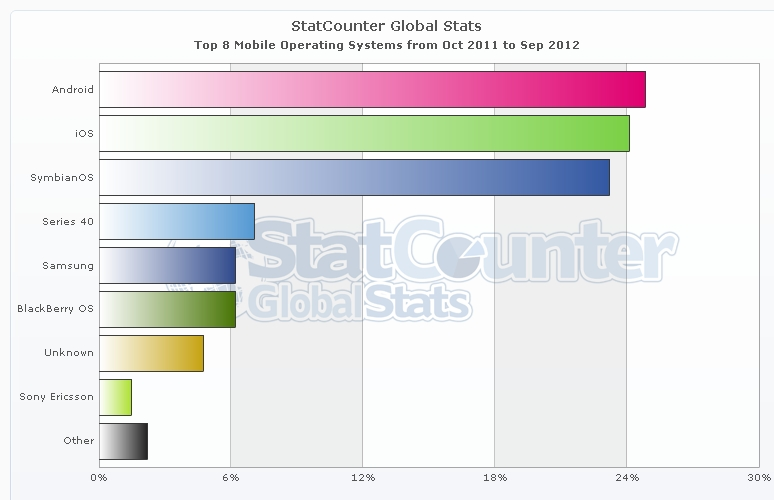
\includegraphics[scale=0.5]{androidpart1.jpg}\\
	\end{center}


%\setcounter{page}{45}
\setcounter{ejemplo}{0}
%\setcounter{chapter}{3}
\chapter{Por qué en Android}
% \rfoot[\fnz{Adaptado de \emph{Machines, Languages and Computation} de Denning, Dennis, Qualitz}]
%       {\fnz{Adaptado de \emph{Machines, Languages and Computation} de Denning, Dennis, Qualitz}}


%\setcounter{page}{60}
% \setcounter{ejemplo}{0}
%\setcounter{chapter}{4}
% \rfoot[\fnz{Adaptado de \emph{Machines, Languages and Computation} de Denning, Dennis, Qualitz}]
%       {\fnz{Adaptado de \emph{Machines, Languages and Computation} de Denning, Dennis, Qualitz}}
%\chapter{Aceptadores y lenguajes de estados finitos}


\setcounter{ejemplo}{0}
%\setcounter{chapter}{5}
%\setcounter{page}{86}
% \rfoot[\fnz{Adaptado de \emph{Machines, Languages and Computation} de Denning, Dennis, Qualitz}]
%       {\fnz{Adaptado de \emph{Machines, Languages and Computation} de Denning, Dennis, Qualitz}}
 \chapter{El mercado móvil y las App's Stores}


%\setcounter{ejemplo}{0}
%\setcounter{chapter}{6}
%\setcounter{page}{110}
% \rfoot[\fnz{Adaptado de \emph{Machines, Languages and Computation} de Denning, Dennis, Qualitz}]
%       {\fnz{Adaptado de \emph{Machines, Languages and Computation} de Denning, Dennis, Qualitz}}

\part{MAEOCS}



\part{Desarrollando aplicaciones en Android}


%\setcounter{ejemplo}{0}
\chapter{Instalando todo lo necesario para empezar}\label{cap:actividad}
% \rfoot[\fnz{Adaptado de \emph{Programming Language Processors} de David Watt}]
%       {\fnz{Adaptado de \emph{Programming Language Processors} de David Watt}}


\chapter{Creando mi primera actividad}



\chapter{Controles básicos}
%\rfoot{} %De aqui en adelante es de R. Lopez ??


%\setcounter{ejemplo}{0}
%\setcounter{chapter}{7}
%\setcounter{page}{148}
\chapter{Controles avanzados}\label{cap:ascendente}

%\input{extra-ascendente}

%\setcounter{ejemplo}{0}
%\setcounter{chapter}{8}
%\setcounter{page}{157}
\chapter{Usando Google Maps}


%\chapter{Ambientes de ejecuci'on}
%\input{runtime}


%\appendix


\end{mainmatter}

% \begin{backmatter}
% \bibliography{lenguajes}
% \printindex
% \end{backmatter}

\end{document}
